% ------------------------------------------------------------------------------
% TYPO3 Version 10.3 - What's New (English Version)
%
% @author	Michael Schams <schams.net>
% @license	Creative Commons BY-NC-SA 3.0
% @link		https://typo3.org/help/documentation/whats-new/
% @language	English
% ------------------------------------------------------------------------------

\section{Changes for Integrators}
\begin{frame}[fragile]
	\frametitle{Changes for Integrators}

	\begin{center}\huge{Chapter 2:}\end{center}
	\begin{center}\huge{\color{typo3darkgrey}\textbf{Changes for Integrators}}\end{center}

\end{frame}

% ------------------------------------------------------------------------------
% Feature | 90333 | Dashboard

\begin{frame}[fragile]
	\frametitle{Changes for Integrators}
	\framesubtitle{Dashboard}

	% decrease font size for code listing
	\lstset{basicstyle=\tiny\ttfamily}

	\begin{itemize}
		\item Dashboard \textit{presets} can be configured for new users or for users who deleted all their dashboards.
		\item This can be used to show a "Getting Started" dashboard by default.
		\item Example TSconfig:

\vspace{-0.4cm}
\begin{lstlisting}
options.dashboard.dashboardPresetsForNewUsers = default, dashboardPreset-myPreset
\end{lstlisting}

		\item Multiple dashboard presets can be defined in a comma separated list.

	\end{itemize}

\end{frame}

% ------------------------------------------------------------------------------
% Important | 89992 | Use New TranslationServer

\begin{frame}[fragile]
	\frametitle{Changes for Integrators}
	\framesubtitle{Localization Management Platform}

	\begin{itemize}
		\item The SaaS solution "\href{https://crowdin.com/}{Crowdin}" is now used as
			the localization/translation management platform for TYPO3.
		\item We encourage everyone to participate and improve the localization.
		\item Crowdin can be used to translate language labels of the TYPO3 core
			as well as of TYPO3 extensions.
		\item Read more about this in the
			\href{https://docs.typo3.org/m/typo3/reference-coreapi/master/en-us/ApiOverview/Internationalization/TranslationServer/Crowdin.html}{TYPO3 documentation}.
	\end{itemize}

	\begin{figure}
		
\includegraphics[width=0.40\linewidth]{ChangesForIntegrators/crowdin-logo.png}
	\end{figure}

\end{frame}

% ------------------------------------------------------------------------------
% Feature | 90266 | Fluid-based templated emails

\begin{frame}[fragile]
	\frametitle{Changes for Integrators}
	\framesubtitle{Fluid-based HTML Emails (1)}

	% decrease font size for code listing
	\lstset{basicstyle=\smaller\ttfamily}

	\begin{itemize}
		\item TYPO3 now supports sending template-based HTML and plain-text emails.
		\item Emails are built by using the Fluid templating engine.
		\item Email templates can be customized by overwriting the paths to the template files:

\vspace{-0.4cm}
\begin{lstlisting}
$GLOBALS['TYPO3_CONF_VARS']['MAIL']['templateRootPaths'][700] =
  'EXT:my_site_extension/Resources/Private/Templates/Email';

$GLOBALS['TYPO3_CONF_VARS']['MAIL']['layoutRootPaths'][700] =
  'EXT:my_site_extension/Resources/Private/Layouts';
\end{lstlisting}

	\end{itemize}

\end{frame}

% ------------------------------------------------------------------------------
% Feature | 90266 | Fluid-based templated emails

\begin{frame}[fragile]
	\frametitle{Changes for Integrators}
	\framesubtitle{Fluid-based HTML Emails (2)}

	\begin{itemize}
		\item Fluid-based templated emails are used for the following components for example:

			\begin{itemize}
				\item Install Tool test email (see example on the next slide).
				\item Workspace notification email on stage change.
				\item Notification email on backend user login.
			\end{itemize}

	\end{itemize}

\end{frame}

% ------------------------------------------------------------------------------
% Feature | 90266 | Fluid-based templated emails

\begin{frame}[fragile]
	\frametitle{Changes for Integrators}
	\framesubtitle{Fluid-based HTML Emails (3)}

	Test email sent from the Install Tool:

	\begin{figure}
		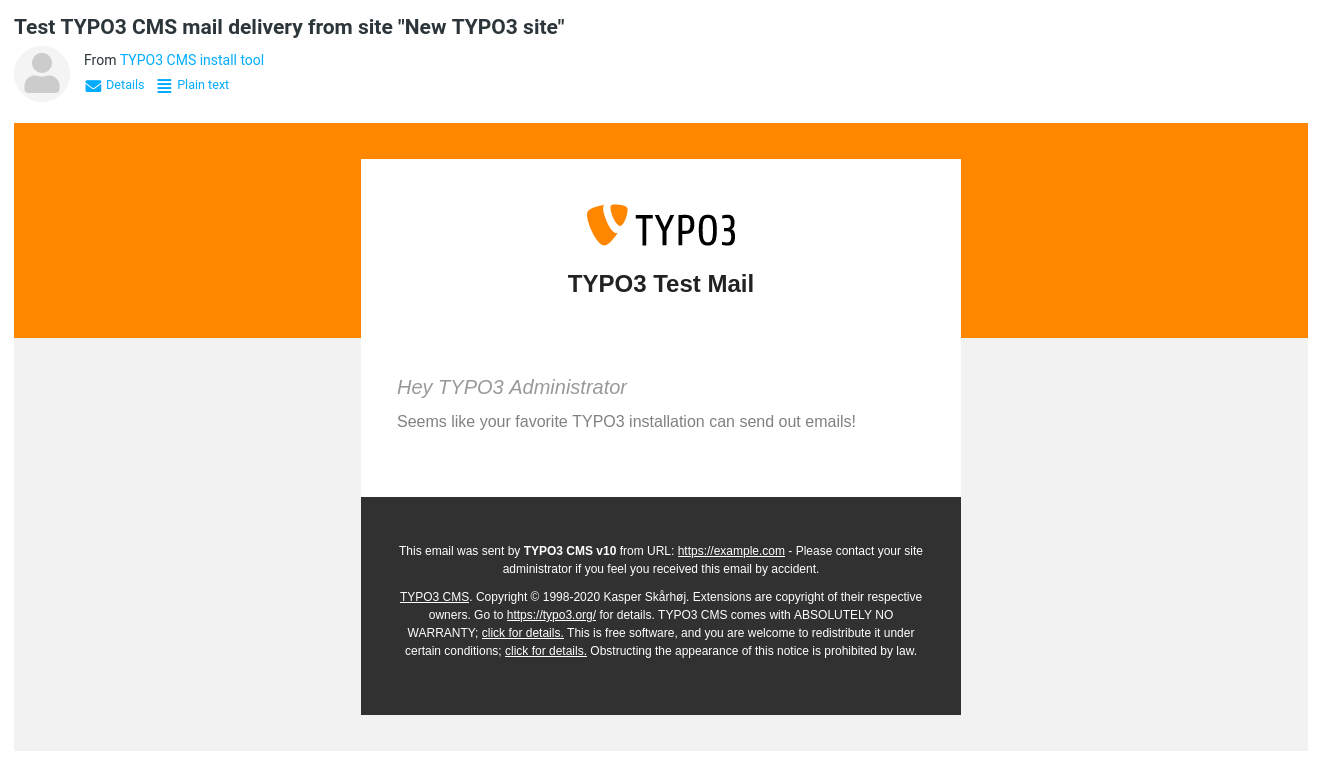
\includegraphics[width=0.8\linewidth]{ChangesForIntegrators/90266-FluidBasedTemplatedEmails.png}
	\end{figure}

\end{frame}

% ------------------------------------------------------------------------------
% Feature | 90203 | Make workspace available in TypoScript conditions

\begin{frame}[fragile]
	\frametitle{Changes for Integrators}
	\framesubtitle{Workspaces and TypoScript}

	% decrease font size for code listing
	\lstset{basicstyle=\smaller\ttfamily}

	\begin{itemize}
		\item A new expression language variable has been added: \texttt{workspace}.
		\item This variable can be used to match a given expression against common workspace parameters.
		\item Currently, the following parameters are supported:\newline
			\small
				\texttt{workspaceId}, \texttt{isLive}, and \texttt{isOffline}.
			\normalsize
		\item For example:

\vspace{-0.4cm}
\begin{lstlisting}
[workspace.workspaceId === 3]
  # Current workspace ID is 3
[end]
\end{lstlisting}

	\end{itemize}

\end{frame}

% ------------------------------------------------------------------------------
% Feature | 88962 | Re-implement old PIDupinRootline TypoScript condition

\begin{frame}[fragile]
	\frametitle{Changes for Integrators}
	\framesubtitle{TypoScript}

	% decrease font size for code listing
	\lstset{basicstyle=\smaller\ttfamily}

	\begin{itemize}
		\item The old \texttt{PIDupinRootline} condition has been re-implemented
			in TypoScript using the Symfony expression language.
		\item Old TypoScript condition syntax:

\vspace{-0.4cm}
\begin{lstlisting}
[PIDupinRootline = 30]
  page.10.value = I'm on any subpage of page with UID 30.
[END]
\end{lstlisting}

		\item New TypoScript condition syntax:

\vspace{-0.4cm}
\begin{lstlisting}
[30 in tree.rootLineParentIds]
  page.10.value = I'm on any subpage of page with UID 30.
[END]
\end{lstlisting}

	\end{itemize}

\end{frame}

% ------------------------------------------------------------------------------
% Feature | 90426 | Browser-native lazy loading for images

\begin{frame}[fragile]
	\frametitle{Changes for Integrators}
	\framesubtitle{Lazy Loading for Images}

	% decrease font size for code listing
	\lstset{basicstyle=\smaller\ttfamily}

	\begin{itemize}
		\item The HTML attribute \texttt{loading} can now be set for \texttt{<img>}-tags.
		\item Browsers which support this feature won't load these images until they are in the viewport.
		\item The behavior can be modified by the following TypoScript constant:

\vspace{-0.4cm}
\begin{lstlisting}
styles.content.image.lazyLoading = lazy
\end{lstlisting}

		\item Valid values are: \texttt{lazy} (default), \texttt{eager}, and \texttt{auto}.
		\item The Fluid \textit{Image-ViewHelper} also supports lazy loading now:

\vspace{-0.4cm}
\begin{lstlisting}
<f:image src="{fileObject}" treatIdAsReference="true"
  loading="lazy" />
\end{lstlisting}

	\end{itemize}

\end{frame}

% ------------------------------------------------------------------------------
% Important | 89869 | Change lockIP default to disabled for both frontend and backend

\begin{frame}[fragile]
	\frametitle{Changes for Integrators}
	\framesubtitle{Default values for \texttt{lockIP}/\texttt{lockIPv6}}

	% decrease font size for code listing
	\lstset{basicstyle=\smaller\ttfamily}

	\begin{itemize}
		\item The default values for \texttt{lockIP} settings have been changed.
		\item The following four system variables are now \textbf{disabled} by default:

			\begin{itemize}
				\item \texttt{[FE]['lockIP']}
				\item \texttt{[FE]['lockIPv6']}
				\item \texttt{[BE]['lockIP']}
				\item \texttt{[BE]['lockIPv6']}
			\end{itemize}

		\item The old default values ("\texttt{4}" for the backend and "\texttt{2}" for the frontend)
			caused problems for example for clients with IPv4 and IPv6 address support.

	\end{itemize}

\end{frame}

% ------------------------------------------------------------------------------
% Feature | 90052 | Form YAML configuration available in configuration module

\begin{frame}[fragile]
	\frametitle{Changes for Integrators}
	\framesubtitle{Form: YAML Configuration}

	\begin{columns}[T]
		\begin{column}{.04\textwidth}
		\end{column}
		\begin{column}{.38\textwidth}

			If the system extension \texttt{EXT:form} is installed, the parsed YAML configuration
			can be displayed under \textbf{SYSTEM} $\rightarrow$ \textbf{Configuration}.

			\vspace{0.2cm}

			This also requires administrators to activate \texttt{EXT:lowlevel} of course.

		\end{column}
		\begin{column}{.58\textwidth}
			\vspace{-0.3cm}
			\begin{figure}
				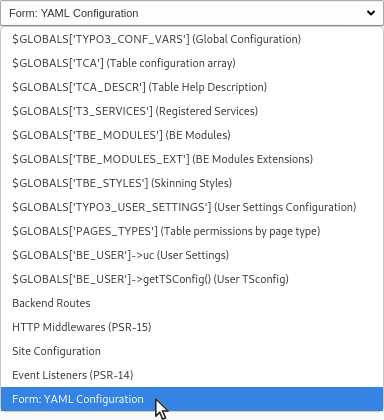
\includegraphics[width=0.70\linewidth]{ChangesForIntegrators/90052-AddYamlConfigurationToConfigurationModule.png}
			\end{figure}
		\end{column}
	\end{columns}

\end{frame}

% ------------------------------------------------------------------------------
% Feature | 88147 | Add possibility to configure the path to sitemap xslFile

\begin{frame}[fragile]
	\frametitle{Changes for Integrators}
	\framesubtitle{SEO: \texttt{Sitemap.xsl}}

	% decrease font size for code listing
	\lstset{basicstyle=\tiny\ttfamily}

	\begin{itemize}
		\item The default path to the file \texttt{Sitemap.xsl} of the system extension
			\texttt{EXT:seo} can be customized now:

\vspace{-0.4cm}
\begin{lstlisting}
# Globally for all sitemaps:
plugin.tx_seo.config.xslFile = EXT:myext/Resources/Public/CSS/mySite.xsl

# For all sitemaps of a specific type:
plugin.tx_seo.config.<sitemapType>.sitemaps.xslFile = EXT:myext/Resources/Public/CSS/mySite.xsl

# For a specific sitemap:
plugin.tx_seo.config.<sitemapType>.sitemaps.<sitemap>.config.xslFile =
  EXT:myext/Resources/Public/CSS/mySite.xsl
\end{lstlisting}

		\item The default path reads:\newline
			\smaller
				\texttt{EXT:seo/Resources/Public/CSS/Sitemap.xsl}
			\normalsize

	\end{itemize}

\end{frame}

% ------------------------------------------------------------------------------
% Feature | 82062 | Progress for Reference Index update on CLI

\begin{frame}[fragile]
	\frametitle{Changes for Integrators}
	\framesubtitle{Reference Index}

	% decrease font size for code listing
	\lstset{basicstyle=\tiny\ttfamily}

	\begin{itemize}
		\item Progress bars are shown for each database table during Reference Index update.
	\end{itemize}

	\begin{figure}
		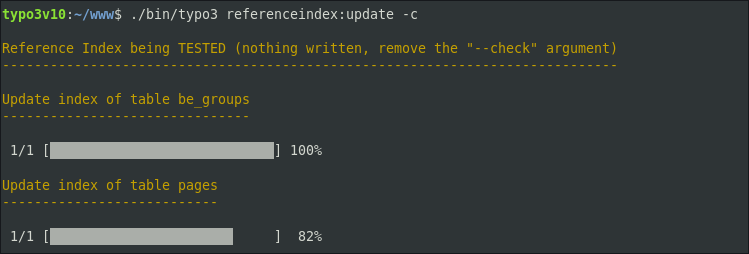
\includegraphics[width=0.85\linewidth]{ChangesForIntegrators/82062-ProgressForReferenceIndexUpdateOnCli.png}
	\end{figure}

\end{frame}

% ------------------------------------------------------------------------------
% Feature | 90425 | Add seo fields to info module

\begin{frame}[fragile]
	\frametitle{Changes for Integrators}
	\framesubtitle{Info Module}

	\begin{itemize}
		\item SEO and Social Media details have been added to the Info module:\newline
			\textbf{WEB} $\rightarrow$ \textbf{Info} $\rightarrow$ \textbf{Pagetree Overview}.
	\end{itemize}

	\begin{figure}
		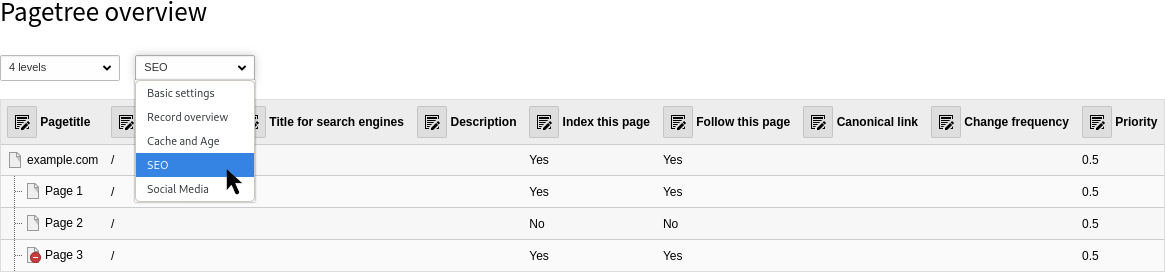
\includegraphics[width=0.85\linewidth]{ChangesForIntegrators/90425-AddSeoFieldsToInfoModule.png}
	\end{figure}

\end{frame}

% ------------------------------------------------------------------------------
% Feature | 59452 | scheduler:run command accepts multiple task options

\begin{frame}[fragile]
	\frametitle{Changes for Integrators}
	\framesubtitle{Scheduler}

	% decrease font size for code listing
	\lstset{basicstyle=\tiny\ttfamily}

	\begin{itemize}
		\item Multiple tasks can be executed when using the option \texttt{-}\texttt{-}\texttt{task}
	\end{itemize}

	\begin{figure}
		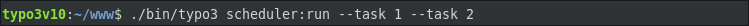
\includegraphics[width=0.85\linewidth]{ChangesForIntegrators/59452a-MultipleTasksInSchedulerCommand.png}
	\end{figure}

	\begin{itemize}
		\item Verbose output can be enabled by \texttt{-}\texttt{v} and \texttt{-}\texttt{vv}
	\end{itemize}

	\begin{figure}
		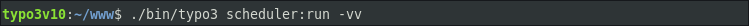
\includegraphics[width=0.85\linewidth]{ChangesForIntegrators/59452b-MultipleTasksInSchedulerCommand.png}
	\end{figure}

\end{frame}

% ------------------------------------------------------------------------------
% Feature | 90298 | Improve user info in BE User module

\begin{frame}[fragile]
	\frametitle{Changes for Integrators}
	\framesubtitle{Backend User Module}

	\begin{itemize}
		\item A new detail view of backend user records shows all relevant data.
		\item Additional fields have been added to the function to compare users.
		\item This function also takes subgroups into account now.
		\item The user interface of the module will be adjusted and optimized further.
		\item These changes make it easier for integrators/administrators to check
			and compare user permissions without switching to the user.
	\end{itemize}

\end{frame}

% ------------------------------------------------------------------------------
% Feature | 89894 | Separate system extensions from 3rd-party extensions visually

\begin{frame}[fragile]
	\frametitle{Changes for Integrators}
	\framesubtitle{Extension Manager}

	System and 3rd-party extensions can now be listed separately in the Extension Manager.

	\begin{figure}
		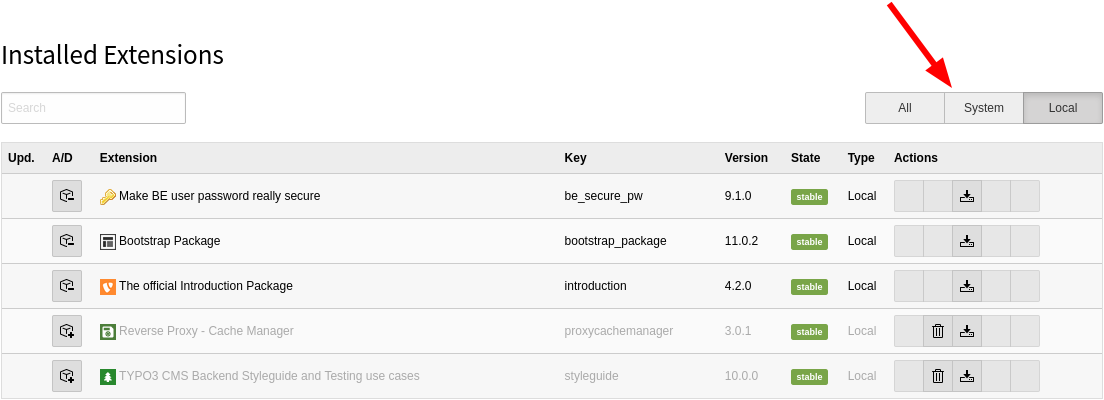
\includegraphics[width=0.9\linewidth]{BackendUserInterface/89894-SeparateSystemExtensionsFrom3rdPartyExtensionsVisually.png}
	\end{figure}

\end{frame}

% ------------------------------------------------------------------------------
% Feature | 90136 | Show application context in the Environment module

\begin{frame}[fragile]
	\frametitle{Changes for Integrators}
	\framesubtitle{Environment Overview}

	The current application context is now shown in the Environment module:\newline
	\textbf{ADMIN TOOLS} $\rightarrow$ \textbf{Environment} $\rightarrow$ \textbf{Environment Overview}.

	\begin{figure}
		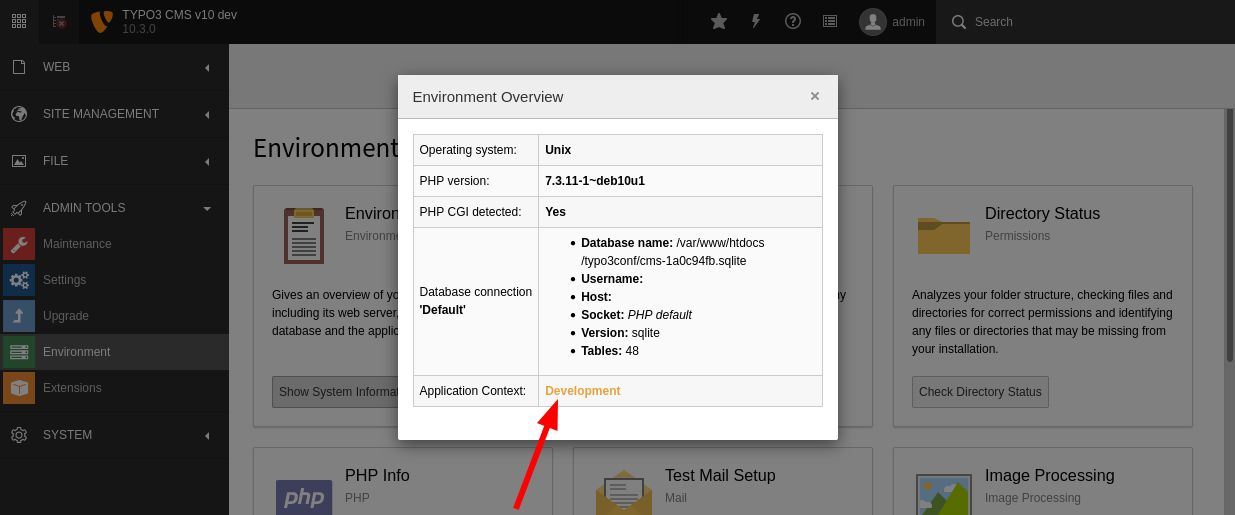
\includegraphics[width=0.9\linewidth]{ChangesForIntegrators/90136-ShowApplicationContextInTheEnvironmentModule.png}
	\end{figure}

\end{frame}

% ------------------------------------------------------------------------------
% Task | 89844 | Improve visual appearance of feature toggles

\begin{frame}[fragile]
	\frametitle{Changes for Integrators}
	\framesubtitle{Feature Toggles}

	The visual appearance of feature toggles has been improved:
	\newline\newline
	\smaller\textbf{TYPO3 < 10.3}\tabto{6cm}\textbf{TYPO3 >= 10.3}\normalsize

	\begin{figure}
		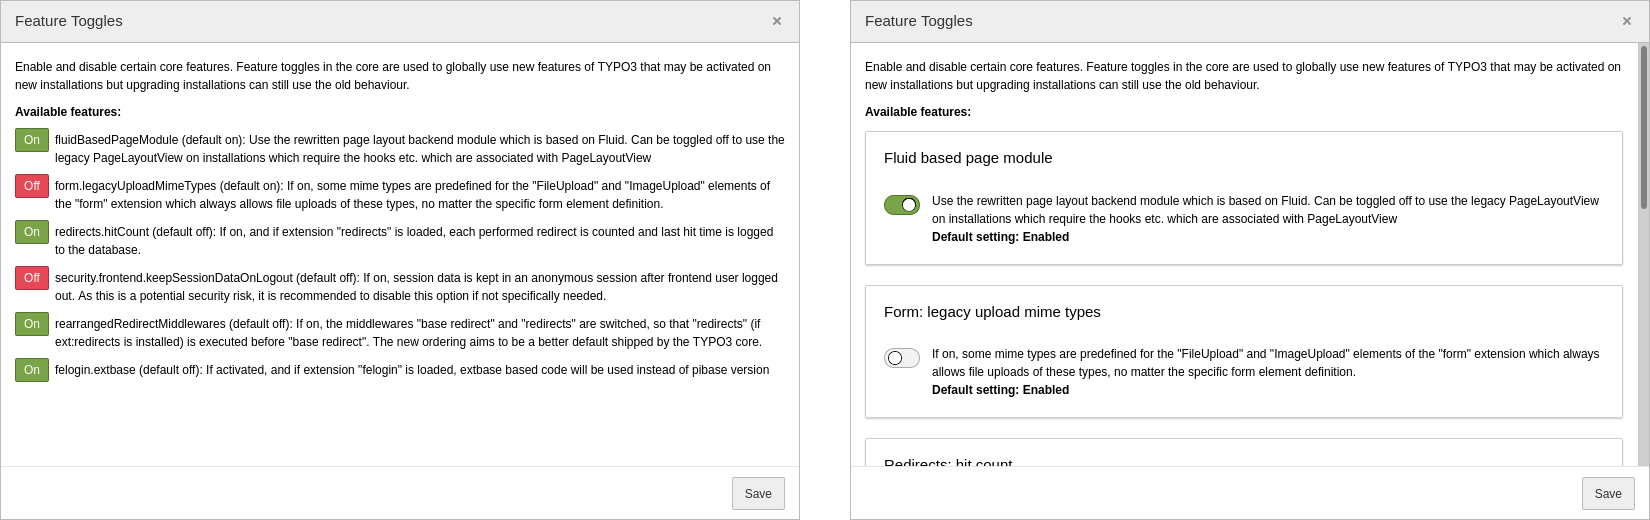
\includegraphics[width=1\linewidth]{ChangesForIntegrators/89844-ImproveVisualAppearanceOfFeatureToggles.png}
	\end{figure}

\end{frame}

% ------------------------------------------------------------------------------
% Feature | 89513 | Provide password recovery for backend users
%
%\begin{frame}[fragile]
%	\frametitle{Changes for Integrators}
%	\framesubtitle{Password Recovery Email}
%
%	\begin{itemize}
%
%		\item Password resets for backend users are only valid for 4 hours.\newline
%			This time limit is not configurable.
%		\item The function can optionally be disabled for all users or for admin users only to strengthen security.
%		\item If users share one email address, an alternative email text is used.
%		\item TCA field \texttt{be\_users.email} must not be set to \texttt{eval=email}.
%
%		\item The function only works for users, who:
%			\begin{itemize}
%				\item have an email address set,
%				\item have a password set, and
%				\item are not disabled/deleted.
%			\end{itemize}
%
%	\end{itemize}
%
%\end{frame}
%
% ------------------------------------------------------------------------------
